% id: 0643
% book: RPM 중3-2 수학 · 06 상관관계
% section: 실력 UP
% figure: crop:fig-0643-2.png
% answer: $25\mkern3mu \%$
% answer_source: 답지
% variant_level: 0 (원본 전사)
% 이 파일은 build.mjs 가 items.json 에서 만든다. 고칠 때는 items.json 을 고친다.
\noindent\begin{minipage}[t]{0.58\linewidth}\vspace{0pt}\raggedright 오른쪽 그림은 경진이네 반 학생 20명의 중간고사와 기말고사 미술 점수에 대한 산점도이다. 다음 조건을 모두 만족시키는 학생들은 전체의 몇 $\%$인지 구하시오.\end{minipage}\hfill\begin{minipage}[t]{0.4\linewidth}\vspace{0pt}\centering \setlength{\dmfigw}{101.8pt}\ifdim\dmfigw>\linewidth\setlength{\dmfigw}{\linewidth}\fi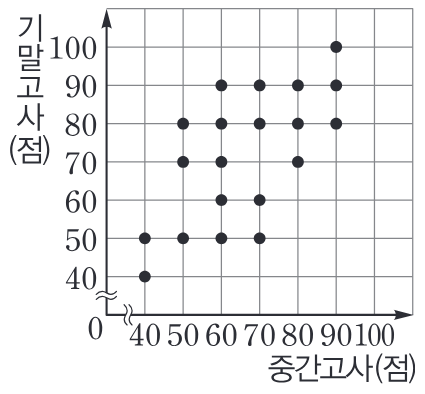
\includegraphics[width=\dmfigw]{figures/fig-0643-2.png}\end{minipage}\par
\par\smallskip\begin{center}\setlength{\dmfigw}{240.4pt}\ifdim\dmfigw>\linewidth\setlength{\dmfigw}{\linewidth}\fi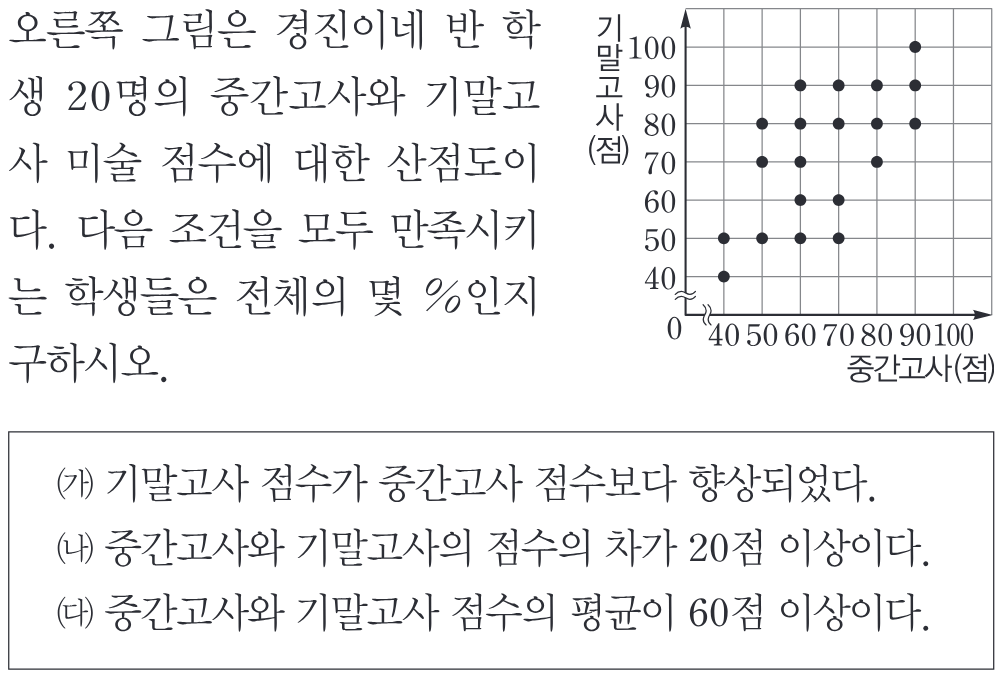
\includegraphics[width=\dmfigw]{figures/fig-0643.png}\end{center}
